\documentclass[11pt]{article}

\usepackage[margin=1in]{geometry}
\usepackage[T1]{fontenc}
\usepackage[utf8]{inputenc}
\usepackage{mathpazo}
\usepackage{microtype}
\usepackage{amsmath,amssymb,amsthm,mathtools}
\usepackage{booktabs,tabularx,array,longtable}
\usepackage{enumitem}
\usepackage{xcolor}
\usepackage[most]{tcolorbox}
\usepackage{tikz}
\usetikzlibrary{arrows.meta,positioning,fit,calc}
\usepackage[round,authoryear]{natbib}
\usepackage[hidelinks]{hyperref}
\usepackage{bookmark}
\usepackage{fancyhdr}

\definecolor{navy}{HTML}{17365D}
\definecolor{bluegray}{HTML}{EAF0F6}
\definecolor{warmgray}{HTML}{F4F1EC}
\definecolor{brick}{HTML}{8A3426}
\definecolor{forest}{HTML}{2F5B45}

\hypersetup{
	pdftitle={Questions Before Priors: Directed Causal Inquiry, Strategic Insight, and the Theory-Based View},
	pdfauthor={Research development memorandum for Michael D. Ryall},
	pdfsubject={Theory-Based View research agenda and first-paper architecture}
}

\setlength{\parindent}{0pt}
\setlength{\parskip}{0.62em}
\setlist[itemize]{topsep=0.25em,itemsep=0.18em,leftmargin=1.5em}
\setlist[enumerate]{topsep=0.25em,itemsep=0.22em,leftmargin=1.7em}
\renewcommand{\arraystretch}{1.18}

\pagestyle{fancy}
\fancyhf{}
\fancyhead[L]{\small Questions Before Priors}
\fancyhead[R]{\small Research memorandum}
\fancyfoot[C]{\thepage}
\setlength{\headheight}{14pt}

\newtheorem{proposition}{Proposition}[section]
\newtheorem{definition}[proposition]{Definition}
\newtheorem{conjecture}[proposition]{Conjecture}
\newtheorem{remark}[proposition]{Remark}

\newtcolorbox{thesisbox}{
	colback=bluegray,
	colframe=navy,
	boxrule=0.7pt,
	arc=1.5mm,
	left=2.5mm,right=2.5mm,top=2mm,bottom=2mm
}
\newtcolorbox{warningbox}{
	colback=warmgray,
	colframe=brick,
	boxrule=0.7pt,
	arc=1.5mm,
	left=2.5mm,right=2.5mm,top=2mm,bottom=2mm
}
\newtcolorbox{designbox}{
	colback=white,
	colframe=forest,
	boxrule=0.7pt,
	arc=1.5mm,
	left=2.5mm,right=2.5mm,top=2mm,bottom=2mm
}

\newcommand{\cplan}{C^{\mathrm{Plan}}}
\newcommand{\cplus}{C^{+}}
\newcommand{\M}{\mathcal{M}}
\newcommand{\F}{\mathcal{F}}
\newcommand{\Lcal}{\mathcal{L}}
\newcommand{\Q}{\mathcal{Q}}
\newcommand{\R}{\mathcal{R}}
\newcommand{\E}{\mathbb{E}}
\newcommand{\Prb}{\mathbb{P}}
\newcommand{\doop}{\operatorname{do}}
\newcommand{\Reach}{\operatorname{Reach}}
\newcommand{\Ext}{\operatorname{Ext}}
\newcommand{\proj}{\operatorname{proj}}

\title{\textbf{Questions Before Priors}\\[0.35em]
	\large Directed Causal Inquiry, Strategic Insight, and a Research Agenda for the Theory-Based View}
\author{Research development memorandum for Michael D. Ryall}
\date{July 2026}

\begin{document}
	\maketitle
	
	\begin{abstract}
		This memorandum consolidates a proposed research program at the intersection of the theory-based view of strategy, causal inference, game theory, unawareness, action theory, and value capture.  Its central claim is that the most important missing object is neither a strategic theory nor a Bayesian belief over theories, but a process of \emph{directed causal inquiry}: experience makes a defect in an existing theory salient; the defect becomes a question; inquiry produces a candidate causal representation; and only then can Bayesian judgment operate on an expanded model space.  The central difficulty is the source of candidate theories.  If they are merely selected from a list the agent already represents, the model describes attention or model selection rather than genuine unawareness.  The memorandum therefore distinguishes retrieval, recombination, abstraction, social transmission, and genuine conceptual expansion; sets out a two-agent causal-game architecture in which agents' theories cause their actions and thereby generate one another's experience; identifies what must remain outside an agent's subjective state space; and proposes a sequence of papers.  It is a design document, not yet a commitment to a particular example or solution to the theory-generation problem.
	\end{abstract}
	
	\begin{thesisbox}
		\textbf{Current organizing thesis.}
		Bayesian reasoning disciplines belief revision and judgment \emph{within} a represented causal language.  A question is a localized representation of a defect in that language.  An insight is a fallible causal representation that was not expressible in the prior language.  The distinctive theoretical task is to explain how experience directs the transition from an unrepresented possibility to a question and then to a new representation without placing the new theory, under another name, in the agent's original hypothesis space.
	\end{thesisbox}
	
	\tableofcontents
	\newpage
	
	\section{Purpose and status of the project}
	
	The theory-based view (TBV) treats economic actors as theorists whose causal understandings shape what they notice, which possibilities they entertain, how they experiment, and what they do \citep{FelinZenger2017,FelinGambardellaZenger2024}.  The developing literature has made substantial progress on theory-guided experimentation, entrepreneurial search, imagination, pivots, and competition among theories \citep{CamuffoEtAl2024,ChavdaGansStern2024,EhrigZenger2024,OttHannah2024,RindovaMartins2024,Sorenson2024}.  Yet the origin of a genuinely novel theory remains incompletely formalized.  Much of the current work begins after the agent already possesses a set of attributes, causal links, hypotheses, or possible futures over which belief and experimentation can operate.
	
	The proposed agenda starts one step earlier.  Its central object is the transition
	\begin{equation}
		\label{eq:cycle}
		\text{experience}
		\longrightarrow
		\text{question}
		\longrightarrow
		\text{insight}
		\longrightarrow
		\text{theory}
		\longrightarrow
		\text{judgment}
		\longrightarrow
		\text{action}
		\longrightarrow
		\text{new experience}.
	\end{equation}
	The transition is recursive: accumulated understanding shapes which experiences are anomalous, which anomalies become questions, and which questions appear answerable.  Heterogeneous prior understanding can therefore generate heterogeneous questions and awareness spaces even when agents observe similar events and have identical preferences or Bayesian competence.
	
	The agenda draws on four existing bodies of work in Ryall's portfolio:
	\begin{enumerate}
		\item \textbf{Pre-Bayesian intelligibility and Lonergan.}  The Utah presentation and the Ryall--Wilkins manuscript distinguish experience, questions for intelligence, insight, formulation, judgment, and decision.  They treat inquiry as a directed search for intelligibility rather than undirected information processing \citep{RyallUtah2025,RyallWilkins2018,Lonergan1992}.
		\item \textbf{Causal theories and ambiguity.}  \citet{Ryall2009} formalizes objective causal structures, faithful probability distributions, observational equivalence, subjective Bayesian ambiguity, and the distinct roles of passive observation and active experimentation.
		\item \textbf{Action, deliberation, and commitment.}  The action-theory appendix develops the agents $C$, $\cplus$, and $\cplan$.  In particular, $\cplus$ deliberately expands an awareness frontier when refinement might change the current action, while $\cplan$ carries forward a sparse, on-plan cache of earlier deliberation \citep{RyallAction2026}.
		\item \textbf{Value creation and capture.}  Value capture theory supplies a disciplined account of how strategic understanding and awareness can translate into competitive payoffs, including environments with incomplete information and unawareness \citep{GansRyall2017,BryanRyallSchipper2022}.
	\end{enumerate}
	
	The project is not yet a claim that the mystery of human conceptual insight has been solved.  The immediate goal is more precise: identify a minimal economic architecture in which experience endogenously generates a \emph{directed question}, distinguish the formation of a question from the arrival of its answer, and state conditions under which a new causal representation counts as an insight rather than a bookkeeping expansion.
	
	\section{The proposed research agenda}
	
	\subsection{One sequence, several paper-sized problems}
	
	The broad program can be summarized as follows.
	
	\begin{center}
		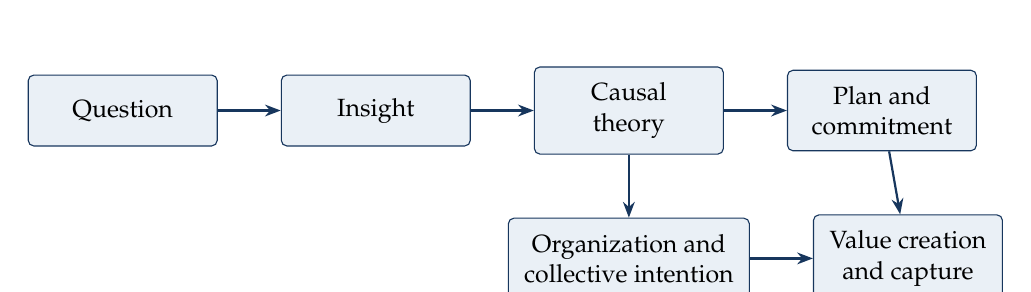
\begin{tikzpicture}[
			node distance=8mm and 8mm,
			every node/.style={font=\small,align=center},
			box/.style={draw=navy,rounded corners=2pt,fill=bluegray,minimum height=9mm,minimum width=24mm,inner sep=2mm},
			arr/.style={-{Stealth[length=2mm]},thick,draw=navy}
			]
			\node[box] (q) {Question};
			\node[box,right=of q] (i) {Insight};
			\node[box,right=of i] (t) {Causal\\theory};
			\node[box,right=of t] (p) {Plan and\\commitment};
			\node[box,below=of t] (o) {Organization and\\collective intention};
			\node[box,right=of o] (v) {Value creation\\and capture};
			\draw[arr] (q)--(i);
			\draw[arr] (i)--(t);
			\draw[arr] (t)--(p);
			\draw[arr] (t)--(o);
			\draw[arr] (p)--(v);
			\draw[arr] (o)--(v);
		\end{tikzpicture}
	\end{center}
	
	Each link can support a separate paper because it involves a different theoretical obstacle.
	
	\begin{description}[style=nextline,leftmargin=1.5em,labelindent=0pt]
		\item[Paper 1: Questions before priors --- directed causal inquiry under unawareness.]
		How can experience reveal that the current causal understanding is defective, localize a worthwhile question, and generate a genuinely new candidate representation?  How are beliefs coherently formed after the representation becomes expressible?  A minimal two-agent causal game makes experience endogenous and allows the other agent's theory to be part of the causal world.
		
		\item[Paper 2: From theory to plan --- commitment under changing awareness.]
		How is a judged causal theory embodied in a plan?  When does the sparse cache of $\cplan$ rationally preserve commitment, and when do anomalies or new insights justify revision?  The central objects are theory-conditioned plans, confirmatory inquiry, off-plan exploration, and the distinction between rational persistence and dogmatism.
		
		\item[Paper 3: The theory-bearing firm.]
		How do individual insights become shared meanings, collective intentions, organizational routines, and an enduring center of agency?  The Ryall--Wilkins account suggests that a firm is not merely a set of contracts or a collection of beliefs; it can become a socially constituted subject that preserves, transmits, and acts through shared causal understanding.
		
		\item[Paper 4: Competing theories and value capture.]
		How do asymmetric causal understandings alter value creation, bargaining possibilities, imitation, resource acquisition, and rents?  This paper would join the front-end process of theory formation to the cooperative-game back end of value capture.  Strategic disclosure, concealment, persuasion, and induced rival unawareness become central.
	\end{description}
	
	Paper 1 is foundational.  If it succeeds, later papers can use its awareness-transition operator rather than stipulating new theories or awareness levels.
	
	\subsection{The agenda's prospective contribution to the TBV}
	
	The TBV has established that theories direct search and action.  The proposed agenda aims to explain three logically prior sources of heterogeneity:
	\begin{enumerate}
		\item agents possess different accumulated understandings and therefore classify the same experiences differently;
		\item those classifications generate different questions and different assessments of answerability; and
		\item different inquiry paths produce different conceptual languages, priors, theories, and strategies.
	\end{enumerate}
	This sequence provides a microfoundation for strategic variety that is neither a random draw of beliefs nor a difference in information processing capacity.  It also makes path dependence endogenous: theories shape actions; actions determine experience; experience determines which questions can arise; and questions determine future theories.
	
	\section{Relevant literature and the exact gap}
	
	\subsection{The theory-based view}
	
	The foundational TBV argument is that theories do more than summarize evidence: they direct attention toward particular causal possibilities, support counterfactual reasoning, and guide experimentation \citep{FelinZenger2017}.  The 2024 \emph{Strategy Science} collection substantially develops this view.  \citet{CamuffoEtAl2024} formalize theory-driven decisions and experimentation; \citet{ChavdaGansStern2024} examine theory-based entrepreneurial search; \citet{Sorenson2024} connects theory, search, and learning; \citet{OttHannah2024} study how entrepreneurs develop a poorly formed thesis into a more elaborate causal model; \citet{RindovaMartins2024} emphasize imagination; and \citet{EhrigZenger2024} model theories as generators of awareness, confidence, resource acquisition, and rents.
	
	These contributions make the proposed project timely rather than redundant.  They establish the importance of theory content, experimentation, and awareness while leaving room for a formal account of the question--insight transition.  In particular, a Bayesian network over selected attributes can model reasoning once the relevant attributes and candidate links are present.  It cannot by itself explain how a new causal predicate, distinction, or actor-type becomes available for representation.
	
	\subsection{Causal inference and active learning}
	
	Causal graphical models separate observational association from intervention and counterfactual reasoning \citep{Pearl2009,SpirtesEtAl2000}.  \citet{Ryall2009} brings this machinery into strategy.  An incumbent's operating structure is a directed acyclic graph; faithful distributions link structure to observed activities; passive experience identifies the empirical distribution and narrows inference to a Markov-equivalence class; and active experience may discriminate among observationally indistinguishable structures.  This is a powerful account of causal learning under a fixed vocabulary.
	
	Active causal-learning methods likewise select interventions to split a represented equivalence class efficiently \citep{HeGeng2008}.  The maintained premise is that the variables and relevant class of graphs are already available.  Thus causal discovery supplies both a benchmark and a boundary.  It explains \emph{closed} causal questions exceptionally well.  It does not explain where a previously unavailable node, category, mechanism, or model of a rival's reasoning comes from.
	
	\subsection{Unawareness, discovery, and changing state spaces}
	
	Standard state-space models cannot represent nontrivial unawareness while retaining familiar knowledge axioms \citep{DekelLipmanRustichini1998}.  Generalized state-space and lattice models represent multiple awareness levels, asymmetric awareness, beliefs, and games \citep{HeifetzMeierSchipper2006,HeifetzMeierSchipper2013}.  These models sharply distinguish an event assigned low or zero probability from an event the agent cannot formulate.
	
	The literature also addresses growing awareness and belief revision.  Reverse Bayesianism preserves appropriate relative odds as the state space expands \citep{KarniViero2013}; awareness of unawareness allows agents to recognize that unspecified consequences may exist \citep{KarniViero2017}; extended Bayesianism incorporates unforeseen evidence into richer probability spaces \citep{Piermont2021}; multiple-prior models represent learning with incomplete awareness and ambiguity \citep{GrantMeneghelTourky2022}; and intertemporal models treat long-horizon decisions with growing awareness \citep{Viero2021}.  Recent work even shows how a decision maker can hold beliefs about the rate of novelty without representing the identities of the novel objects \citep{Schipper2025}.
	
	\citet{Schipper2021} distinguishes learning, which discards conceived possibilities, from discovery, which adds possibilities not previously conceived.  In discovery processes, play in a game with unawareness can reveal actions and move players to a richer game.  This is the closest formal neighbor to the proposed project.  It also clarifies the remaining gap: the discovery transition specifies how play exposes an objectively available action; it does not generally explain the endogenous construction of a causal concept or theory that makes an otherwise puzzling history intelligible.
	
	\subsection{What is not yet joined}
	
	The neighboring literatures solve different pieces:
	
	\begin{center}
		\small
		\begin{tabularx}{\textwidth}{@{}p{0.19\textwidth}X X@{}}
			\toprule
			\textbf{Literature} & \textbf{What it supplies} & \textbf{What remains for this project} \\
			\midrule
			TBV & Theories direct attention, search, experimentation, and action. & Endogenous question formation and genuinely novel causal representation. \\
			Causal discovery & Bayesian learning over DAGs, equivalence classes, identifiability, and interventions. & Expansion of the variable and model language. \\
			Unawareness & Multiple awareness spaces, interactive beliefs, discovery, and coherent updating over expanding spaces. & Why a particular experience generates a particular causal question and candidate theory. \\
			Action theory & Costly directed expansion, planning, and rational commitment. & The semantic content and genesis of what awareness expansion reveals. \\
			Value capture & Competitive payoff consequences of information, beliefs, and awareness. & A front-end theory of how heterogeneous awareness and theories arise. \\
			\bottomrule
		\end{tabularx}
	\end{center}
	
	\section{The first paper's central problem}
	
	\subsection{Three distinct epistemic operations}
	
	The first paper must not collapse the following problems.
	
	\begin{center}
		\small
		\begin{tabularx}{\textwidth}{@{}p{0.20\textwidth}p{0.24\textwidth}X@{}}
			\toprule
			\textbf{Operation} & \textbf{Fixed objects} & \textbf{Appropriate formal treatment} \\
			\midrule
			Parameter learning & Variables and causal graph & Bayesian updating of mechanism parameters. \\
			Causal-structure learning & Variable vocabulary & Bayesian model selection over DAGs, observational equivalence, and intervention design. \\
			Conceptual expansion & Neither the complete vocabulary nor the complete model class & A pre-Bayesian awareness transition, followed by construction of a prior on the expanded model space. \\
			\bottomrule
		\end{tabularx}
	\end{center}
	
	The 2009 causal-ambiguity model occupies the second row.  The new paper begins where that model's entrant can no longer say, ``the true structure is one of these graphs.''
	
	\subsection{Closed and open causal questions}
	
	\begin{definition}[Closed causal question]
		Given an agent's current model set $\M_{it}$, a closed question $q$ is a represented partition $\{M^a:a\in A(q)\}$ of some subset of $\M_{it}$.  The agent can name or otherwise distinguish the possible answers $a\in A(q)$ and assign beliefs to them.
	\end{definition}
	
	A closed question can be answered through Bayesian experimentation when a feasible intervention induces different likelihoods across its answer cells.  ``Is the remaining edge $X-Y$ oriented $X\to Y$ or $Y\to X$?'' is the canonical example.
	
	\begin{definition}[Open causal question]
		An open question is a tuple
		\begin{equation}
			q=(r_q,\tau_q,\mathcal I_q,R_q),
		\end{equation}
		where $r_q$ identifies a defect or explanandum in the current causal representation, $\tau_q$ describes only a coarse type of completion, $\mathcal I_q$ is a feasible class of inquiry activities, and $R_q$ states what an adequate completion must accomplish.  The agent does not possess a subjective answer set whose members express the semantic contents of the possible completions.
	\end{definition}
	
	An open question is a \emph{causal socket}.  The agent can ask what explains an instability in a particular outcome module without representing the missing cause.  It is a localized awareness of incompleteness, not awareness of the answer.
	
	\subsection{The difficult temporal pivot}
	
	The model should explicitly distinguish three moments:
	\begin{enumerate}
		\item \textbf{Absolute unawareness.}  The agent has no event, question, or placeholder referring to the omitted causal content.
		\item \textbf{Localized awareness of incompleteness.}  Experience reveals a defect in the current account.  The agent can now ask an open question about that defect but cannot formulate its answer.
		\item \textbf{Conceptual awareness.}  Inquiry yields a predicate, variable, mechanism, or rival type that makes a candidate answer expressible.
	\end{enumerate}
	
	Thus the proposal does not claim that directed inquiry begins under total unawareness.  The question is the transition from total unawareness to awareness of unawareness.  Insight is the later transition from an open slot to semantic content.  This distinction should be front and center in any presentation to an economic theorist of unawareness.
	
	\section{A two-agent architecture}
	
	\subsection{The objective causal game}
	
	Let $N=\{1,2\}$ be two strategic agents.  The analyst describes an objective, dynamic structural causal game
	\begin{equation}
		\Gamma^*=
		\left(N,X^*,\{A_i^*\}_{i\in N},F^*,\{O_i^*,u_i\}_{i\in N},\{\Psi_i^*\}_{i\in N}\right).
	\end{equation}
	The objective state contains physical, market, and epistemic components:
	\begin{equation}
		s_t^*=(x_t,\chi_{1t},\chi_{2t}),
		\qquad
		\chi_{it}=(L_{it},M_{it},\mu_{it},P_{it}).
	\end{equation}
	Here $x_t$ collects non-epistemic conditions; $L_{it}$ is agent $i$'s causal language; $M_{it}$ is her current subjective causal theory or model class; $\mu_{it}$ is her belief state; and $P_{it}$ is a current plan or policy representation.  The analyst may represent objects of which either agent is unaware.  Analyst-level representation does not itself imply subjective awareness.
	
	Agent $i$'s strategic action is caused by her theory, information, beliefs, and plan:
	\begin{equation}
		a_{it}=\sigma_i(h_{it};\chi_{it}).
	\end{equation}
	Joint actions and the objective state generate outcomes and future physical states:
	\begin{equation}
		(y_t,x_{t+1})=F^*(x_t,a_{1t},a_{2t},\varepsilon_{t+1}).
	\end{equation}
	Agents observe different projections of this process.  Their experiences may alter beliefs, questions, languages, and later actions.  Time indexing prevents causal circularity: agent 1's current theory causes her current action, which becomes part of agent 2's new experience and may change agent 2's future theory.
	
	The strategically distinctive pathway is
	\begin{equation}
		a_{1t}
		\longrightarrow
		O_{2t}
		\longrightarrow
		\chi_{2,t+1}
		\longrightarrow
		a_{2,t+1}
		\longrightarrow
		u_{1,t+1},
	\end{equation}
	with an analogous path from agent 2 to agent 1.  Structural causal games provide compatible machinery for representing decisions, interventions, strategic relevance, and counterfactuals \citep{HammondEtAl2023}.
	
	\subsection{Raw episodes and represented experience}
	
	Let $z_{it}$ denote agent $i$'s raw episode at time $t$: the perceptual and mnemonic trace of observed actions, contexts, and outcomes.  Her current language supplies a representation map
	\begin{equation}
		r_{it}:z_i^{\le t}\longrightarrow S_{it},
	\end{equation}
	which induces a partition $\Pi_{it}$ and a subjective event algebra $\F_{it}$.  Before insight, all consciously available acts, beliefs, and questions must be measurable with respect to $\F_{it}$.  Two raw episodes can therefore be distinct at the analyst level yet belong to the same conceptual cell for the agent.
	
	This separation is essential to the Lonerganian idea that a person can encounter and remember particulars without yet possessing the universal concept that organizes them.  It is also delicate.  If the agent can already condition her action on a raw feature, that feature is behaviorally represented and cannot later be advertised as genuinely new.  Genuine pre-insight unawareness therefore requires
	\begin{equation}
		\sigma_{it}(z)=\sigma_{it}(z')
		\quad\text{whenever}\quad
		r_{it}(z)=r_{it}(z').
	\end{equation}
	
	\subsection{Bayesian learning inside current awareness}
	
	Let $\M(L_{it})$ be the set of causal models expressible in $L_{it}$.  The agent holds a prior or posterior $\mu_{it}\in\Delta(\M(L_{it}))$.  When a new observation $d_{i,t+1}$ is representable in $L_{it}$, ordinary Bayesian updating gives
	\begin{equation}
		\mu_{i,t+1}^{B}(m)
		=
		\frac{\Prb_m(d_{i,t+1}\mid h_{it},a_t)\mu_{it}(m)}
		{\sum_{\widetilde m\in\M(L_{it})}
			\Prb_{\widetilde m}(d_{i,t+1}\mid h_{it},a_t)\mu_{it}(\widetilde m)}.
	\end{equation}
	Agent $i$ chooses an action to maximize subjective expected payoff given this belief, subject eventually to deliberation costs and plan constraints:
	\begin{equation}
		a_{it}\in\arg\max_{a\in A_i(L_{it})}
		\E_{\mu_{it}}\bigl[u_i\mid a,h_{it}\bigr].
	\end{equation}
	This layer nests the 2009 causal-ambiguity model.  Passive data may concentrate belief on an observational-equivalence class; active inquiry can be valuable when surviving models imply different optimal interventions.
	
	\subsection{Gap detection}
	
	Experience can indicate that the current theory class is inadequate in at least three ways:
	\begin{enumerate}
		\item \textbf{Residual causal ambiguity:} represented models fit passive experience but disagree about action-relevant interventions.
		\item \textbf{Model failure:} no sufficiently simple represented model preserves required conditional independencies, predictive adequacy, or cross-context invariance.
		\item \textbf{Strategic surprise:} the other agent's response is inconsistent with every represented rival type, information structure, or response mechanism.
	\end{enumerate}
	
	Let $v$ index a represented causal module and let
	\begin{equation}
		D_{it}(v)
		=
		\alpha\,\mathrm{PredFail}_{it}(v)
		+\beta\,\mathrm{InvFail}_{it}(v)
		+\gamma\,\mathrm{ActionSep}_{it}(v)
	\end{equation}
	be a provisional defect statistic.  It should not remain an arbitrary weighted score in the final theory.  The desired result is to derive the diagnostic value of its components from restrictions such as modularity, sparsity, repeated regimes, and feasible interventions.  A module enters the question frontier only when the experienced defect exceeds an endogenous or statistically disciplined threshold.
	
	The question generator is therefore a correspondence
	\begin{equation}
		\Q_{it}=G_i(L_{it},M_{it},\mu_{it},h_{it},P_{it}),
	\end{equation}
	not a primitive universal collection of sentences.  It returns a finite set of localized causal sockets.
	
	\subsection{Inquiry and question ranking}
	
	An agent cannot compute ordinary expected value of information over semantically unrepresented answers.  Three weaker forms of evaluation are available:
	\begin{enumerate}
		\item a dominance or partial-order rule based on defect strength, strategic leverage, resolvability, and cost;
		\item robust payoff envelopes adapted from the refinement logic of $\cplus$; or
		\item a meta-belief about whether inquiry will produce a useful novel representation, without a belief over the identity of that representation.
	\end{enumerate}
	
	For the third approach, define
	\begin{equation}
		p_{it}^Q(q)=
		\Prb_i\{\text{inquiry into }q\text{ produces a usable causal completion}\mid\phi_{it}(q)\},
	\end{equation}
	where $\phi_{it}(q)$ contains only currently represented question features: recurrence, localization, analogy to previously solved problems, availability of interventions, and estimated complexity.  This is a prior over \emph{inquiry yield}, not over the semantic answers.  Schipper's delabeled treatment of novelty suggests that such meta-beliefs need not imply awareness of the objects that may appear \citep{Schipper2025}.
	
	A provisional question index is
	\begin{equation}
		I_{it}(q)=p_{it}^{Q}(q)B_{it}(q)-c_{it}(q),
	\end{equation}
	where $B_{it}(q)$ is a subjective, robust measure of the extent to which successful resolution could overturn the current action or plan.  $B_{it}(q)$ is the natural point of contact with $\cplus$: inquiry is valuable because some refinement of a frontier could alter the present choice.  The bounds must be subjective and potentially wrong; exact knowledge of objective consequences behind an unconceived answer would bake awareness into the model.
	
	\subsection{The representation-generating transition}
	
	At the analyst level, inquiry is followed by a representation-generating technology
	\begin{equation}
		\label{eq:Psi}
		(L_{i,t+1}^{0},\iota_{i,t+1})
		=
		\Psi_i^*(L_{it},h_{it}^{\mathrm{raw}},q_{it},e_{it},\eta_{i,t+1}),
	\end{equation}
	where $e_{it}$ is an inquiry action, $\eta_{i,t+1}$ is stochastic, and $\iota_{i,t+1}$ is a candidate new distinction or causal representation.  The superscript $*$ is important: $\Psi_i^*$ is part of the analyst's account of cognition and encounter, not a menu over which the agent can optimize by naming its outputs.
	
	The operator must allow four outcomes:
	\begin{enumerate}
		\item no new representation;
		\item a novel but causally irrelevant distinction;
		\item a plausible but false causal representation; and
		\item a useful causal insight.
	\end{enumerate}
	If asking the correct question automatically reveals the true missing mechanism, the model is only an awareness bookkeeping device.
	
	\subsection{Insight, formulation, and judgment}
	
	\begin{definition}[Candidate causal insight]
		Relative to language $L_{it}$ and open question $q$, an output $\iota$ of \eqref{eq:Psi} is a candidate causal insight if:
		\begin{enumerate}[label=(\roman*)]
			\item \emph{novelty:} $\iota$ is not definable or measurable in $L_{it}$;
			\item \emph{empirical organization:} adding $\iota$ materially reduces the defect targeted by $q$;
			\item \emph{causal content:} the expanded theory produces at least one new intervention or counterfactual implication; and
			\item \emph{minimality:} no proper subextension produces the same causal repair.
		\end{enumerate}
	\end{definition}
	
	An insight is not yet knowledge.  Formulation closes the candidate under its causal implications and produces an expanded model class $\M(L_{i,t+1})$.  Judgment evaluates the candidate using further evidence.  A \emph{strategic insight} is one whose articulated implications change the ranking of actions or plans for a nonempty region of beliefs.
	
	This preserves the Lonerganian distinction.  Equating insight with a posterior threshold would eliminate the difference between grasping a possible intelligibility and judging that it is so.
	
	\subsection{Constructing a prior after insight}
	
	Let $\rho_i:\M(L_{i,t+1})\to\M(L_{it})$ project expanded models onto their old descriptions.  A bridge prior can be written as
	\begin{equation}
		\label{eq:bridge}
		\mu_{i,t+1}^{0}(m')
		=
		\mu_{it}\!\left(\rho_i(m')\right)
		\kappa_{\iota_i}\!\left(m'\mid\rho_i(m')\right).
	\end{equation}
	This form preserves the old marginal distribution while the within-fiber kernel $\kappa_{\iota_i}$ allocates credibility among newly expressible refinements.  Reverse Bayesianism can discipline the preservation of old relative odds when awareness expansion carries no diagnostic evidence \citep{KarniViero2013}.  It does not uniquely determine $\kappa_{\iota_i}$, nor should it.
	
	If anomalous experience both generated the insight and bears on its truth, strict preservation of old odds may be inappropriate.  A clean first treatment should separate discovery data $D^G$ from validation data $D^V$:
	\begin{equation}
		\mu_{i,t+1}(m')
		\propto
		\Prb_{m'}(D^V\mid D^G,\iota_i)
		\mu_{i,t+1}^{0}(m').
	\end{equation}
	Alternatively, the likelihood must condition on the model-generation event.  Naively reusing the same data to generate and confirm the insight would overstate judgmental confidence.
	
	\subsection{The full within-period and intertemporal sequence}
	
	The two-agent process can now be summarized.
	
	\begin{center}
		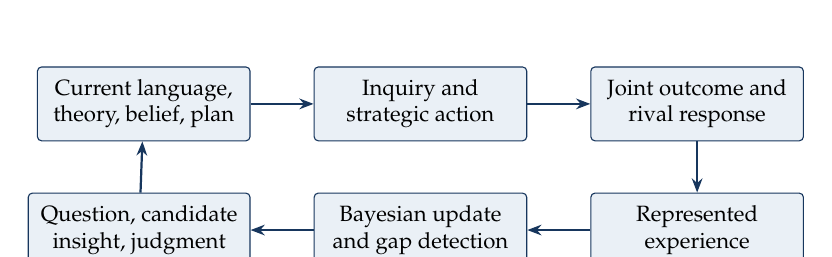
\begin{tikzpicture}[
			node distance=6.5mm and 8mm,
			every node/.style={font=\footnotesize,align=center},
			box/.style={draw=navy,rounded corners=1.5pt,fill=bluegray,minimum height=8mm,minimum width=27mm,inner sep=1.6mm},
			arr/.style={-{Stealth[length=1.8mm]},thick,draw=navy}
			]
			\node[box] (theory) {Current language,\\theory, belief, plan};
			\node[box,right=of theory] (action) {Inquiry and\\strategic action};
			\node[box,right=of action] (joint) {Joint outcome and\\rival response};
			\node[box,below=of joint] (exp) {Represented\\experience};
			\node[box,left=of exp] (gap) {Bayesian update\\and gap detection};
			\node[box,left=of gap] (ins) {Question, candidate\\insight, judgment};
			\draw[arr] (theory)--(action);
			\draw[arr] (action)--(joint);
			\draw[arr] (joint)--(exp);
			\draw[arr] (exp)--(gap);
			\draw[arr] (gap)--(ins);
			\draw[arr] (ins)--(theory);
		\end{tikzpicture}
	\end{center}
	
	Both agents may in principle undergo this process.  For the first formal results, it will probably be wise to hold one agent's awareness-transition technology fixed while analyzing the other's, and then establish a symmetric extension.  The architecture is two-agent even if the first theorem is proved for a focal inquirer facing a strategically responsive rival.
	
	\section{Where do new causal theories come from?}
	
	This is the make-or-break issue.  If the new theory is simply retrieved from an agent's original set of possibilities, then the agent was uncertain, inattentive, or computationally limited---not unaware.  If a model gives every open question an answer set containing the truth, and gives the agent probabilities on that set, the model has converted unawareness into ordinary Bayesian model selection.
	
	\subsection{A taxonomy of apparent novelty}
	
	\begin{center}
		\small
		\begin{tabularx}{\textwidth}{@{}p{0.18\textwidth}X p{0.25\textwidth}@{}}
			\toprule
			\textbf{Source} & \textbf{Description} & \textbf{Status relative to unawareness} \\
			\midrule
			Retrieval & A represented theory was inactive or outside attention and becomes salient. & Not genuine unawareness; an attention model. \\
			Recombination & Known concepts and mechanisms are assembled in a previously unconsidered way. & May be logical non-omniscience; genuine only if the composite was not in the subjective language or act domain. \\
			Abstraction & A new predicate or category is extracted from experienced particulars. & Most promising route to genuinely new semantic awareness. \\
			Analogy or transfer & A causal schema from another domain is mapped onto the present problem. & Can create a new local representation, though the schema itself was known. \\
			Social transmission & Another agent supplies a concept, distinction, or question. & Genuine discovery for the recipient, but postpones the origin problem for the sender. \\
			Exogenous revelation & The environment directly exposes a new action, consequence, or object. & Standard and legitimate in unawareness models, but not yet a theory of insight. \\
			\bottomrule
		\end{tabularx}
	\end{center}
	
	The recommended first-paper mechanism is \emph{contrastive abstraction}, possibly assisted by analogy.  Current concepts pool raw episodes.  Repeatedly contrasting outcomes under comparable actions reveals that the pooled category is not causally homogeneous.  Inquiry searches for a minimal new predicate that splits the category and restores interventional stability.  The new predicate was not an element of the agent's prior event algebra even though the analyst can describe the raw episodes from which it is abstracted.
	
	\subsection{Why analyst-level availability is not subjective awareness}
	
	Every formal unawareness model requires the analyst to describe more than an unaware agent can describe.  A lattice of awareness spaces, for example, is an analyst-level object.  The relevant test is not whether the modeler can name the future theory; it is whether the agent could refer to it, condition an act on it, or assign it a probability before discovery.
	
	This suggests a behavioral non-awareness condition:
	\begin{equation}
		\begin{aligned}
			\iota&\notin\F_{it},\\
			A_i(L_{it})&\text{ contains no act contingent on }\iota,\\
			\mu_{it}&\text{ is not defined on propositions involving }\iota.
		\end{aligned}
	\end{equation}
	The range of $\Psi_i^*$ may be specified by the analyst without appearing in the agent's optimization problem.  In particular, agent $i$ must not choose an inquiry policy by calculating expected utility separately for each future semantic output of $\Psi_i^*$.  Doing so would reintroduce subjective awareness through the back door.
	
	\begin{warningbox}
		\textbf{The unavoidable primitive.}
		No formal model can derive a semantically new concept from literally nothing.  It must specify some representational capacity: a grammar, abstraction operator, analogical repertoire, social transmission process, or environmental disclosure technology.  The contribution cannot be ``creativity without primitives.''  It must instead show how experience \emph{directs} a limited, fallible representation-generating capacity and why that capacity does not amount to a prior over all future theories.
	\end{warningbox}
	
	\subsection{Constructive repertoire without a subjective answer menu}
	
	Let $\R_{it}$ be the analyst's description of operations available to agent $i$: comparison, partition refinement, introduction of a latent common-cause placeholder, analogy, compositional linking, and so forth.  Define
	\begin{equation}
		\Ext_{\R_{it}}(M_{it},q)
	\end{equation}
	as the set of representations that could be constructed through those operations.  This is not necessarily an agent-represented set.  It describes the support of a cognitive production technology, much as a biological production function can describe outcomes that the organism does not anticipate.
	
	A candidate insight might solve
	\begin{equation}
		\iota
		\in
		\arg\min_{\eta\in\Ext_{\R_{it}}(M_{it},q)}
		\left\{-\ell(D^G;M_{it}\oplus\eta)
		+\lambda C_{\R_{it}}(\eta)\right\},
	\end{equation}
	subject to a causal-invariance or counterfactual-content requirement.  The optimization is an analyst's characterization of the output of a constructive process, not necessarily a consciously solved problem by the agent.  Search can terminate prematurely, return a local repair, or fail entirely.
	
	\subsection{The strongest likely objection and response}
	
	An unawareness theorist may object:
	\begin{quote}
		If the agent knows that inquiry into $q$ may produce a missing cause and assigns a value to that possibility, she is already aware of the relevant possibility.  If she does not know this, why would she inquire?
	\end{quote}
	
	The proposed response has two parts.
	
	First, the object of awareness can be \emph{delabeled}.  The agent can recognize that her account is incomplete, or that further inquiry may yield a new distinction, without being able to describe that distinction.  The recent theory of beliefs about novelty provides a formal precedent: one may form beliefs about the occurrence of a new object without representing its identity \citep{Schipper2025}.  Karni and Vier\o's awareness-of-unawareness framework supplies another precedent \citep{KarniViero2017}.
	
	Second, awareness is temporal.  Before the anomaly, the agent need not possess even the localized placeholder.  Experience creates the open question and thereby produces awareness of unawareness.  Inquiry does not operate from absolute unawareness; it operates from a newly recognized gap.  The semantic answer remains outside the agent's language until insight.
	
	This does not eliminate every philosophical difficulty.  It does, however, give a precise position that can be evaluated: \emph{questions represent locations and standards of missing explanation, not the missing semantic contents themselves.}
	
	\section{Potential propositions for the first paper}
	
	The paper needs results that depend on the structure above, not only definitions.
	
	\subsection{Bayesian boundary and nonunique extension}
	
	\begin{proposition}[No Bayesian emergence]
		If the agent's current awareness is represented by $\F_{it}$ and Bayesian conditioning is applied to any event in $\F_{it}$, the posterior remains a probability measure on $\F_{it}$.  Conditioning alone cannot make an event in $\F_{i,t+1}\setminus\F_{it}$ expressible.
	\end{proposition}
	
	\begin{proposition}[Nonuniqueness of the new prior]
		Given a projection from an expanded model space to the old model space, there are generally many expanded priors with the same old marginal.  A reverse-Bayesian consistency condition does not uniquely determine the within-fiber kernel in \eqref{eq:bridge}.
	\end{proposition}
	
	These are boundary results, not the paper's main payoff.  They establish why the pre-Bayesian transition is necessary.
	
	\subsection{Experience localizes inquiry}
	
	The principal substantive result should use a sparse, modular environment.  Suppose the current representation pools two objective causal states and there is a single omitted distinction responsible for a stable difference in interventional response.  Under repeated comparable interventions, the failure of invariance should localize the defect to a specific represented cell or Markov neighborhood.
	
	\begin{conjecture}[Contrastive localization]
		Under a single omitted causal distinction, stable mechanisms outside its causal neighborhood, and sufficiently discriminating experience, the posterior-predictive or invariance-failure pattern identifies a finite question frontier containing the affected module with probability approaching one.
	\end{conjecture}
	
	This is the formal content behind the claim that experience directs inquiry.  It reduces the problem from uniform search over possible theories to local repair without revealing the repair's semantic content.
	
	\subsection{Question value is not information quantity}
	
	\begin{conjecture}[Strategic action separation]
		A causal question has zero strategic refinement value when every causally adequate completion supports the same optimal action, even if the question has high statistical entropy.  Conversely, a low-entropy question can have high value when its answer cells support different optimal actions.
	\end{conjecture}
	
	This proposition ties TBV inquiry to strategic stakes and supplies the proper role for $\cplus$.
	
	\subsection{Self-confirming unawareness}
	
	Because theories cause actions and actions generate experience, the equilibrium path may never produce the contrast required to reveal a gap.
	
	\begin{conjecture}[Awareness trap]
		There exist two-agent causal games in which each agent's current theory is Bayes-consistent with all on-path observations and supports a stable action profile, yet an unrepresented causal distinction would support a profitable deviation.  The distinction remains undiscovered because the current profile never generates the experience required to formulate the relevant question.
	\end{conjecture}
	
	An inquiry action or strategic perturbation may break the trap.  But inquiry can also be performative: if the rival observes the experiment and updates her own theory, the experiment changes the mechanism being studied.  The most statistically revealing inquiry may therefore be strategically inferior.  This is one way the game-theoretic component can provide genuine bite rather than decorative context.
	
	\subsection{Path-dependent theory heterogeneity}
	
	Different prior languages and constructive repertoires imply different representations of identical raw histories.  The agents may therefore detect different gaps, ask different questions, construct different insights, and form different priors.  Persistent strategic heterogeneity can arise without preference heterogeneity, random belief endowments, or differential Bayesian sophistication.
	
	\section{No-baked-in requirements}
	
	The first paper should be evaluated against the following checklist.
	
	\begin{enumerate}
		\item \textbf{No grand subjective hypothesis space.}  The agent must not begin with a prior over all objective causal theories or all outputs of the representation generator.
		\item \textbf{No universal primitive question set.}  Questions must be generated by defects in the current representation, not drawn from an exogenous infinity of sentences.
		\item \textbf{No automatic truth revelation.}  Inquiry can fail, return a false insight, or yield multiple causally adequate candidates.
		\item \textbf{No objective payoff foresight behind unawareness.}  Refinement bounds must be subjective, coarse, and possibly miscalibrated.
		\item \textbf{No passive identification of causal direction without assumptions.}  Identification must respect observational equivalence, hidden variables, and the need for intervention or multiple regimes.
		\item \textbf{No semantic conditioning before awareness.}  Pre-insight actions and beliefs cannot be contingent on the new concept.
		\item \textbf{No optimization across a discovery supergame whose states the agent cannot conceive.}  Inquiry choice can use represented question features or delabeled novelty, not expected utilities indexed by named future theories.
		\item \textbf{No naive double use of experience.}  Evidence that generated a candidate insight must be separated from, or properly conditioned in, the evidence used for judgment.
		\item \textbf{No exogenous rival behavior.}  In the two-agent model, rival responses depend on rival theory and can change when inquiry or strategic actions are observed.
		\item \textbf{No claim to explain creativity ex nihilo.}  The representational repertoire must be stated and its limits acknowledged.
	\end{enumerate}
	
	Passing this checklist does not guarantee a compelling theory.  Failing it would turn the model into ordinary Bayesian learning, bounded attention, or awareness bookkeeping.
	
	\section{Recommended scope of the first paper}
	
	\begin{designbox}
		\textbf{Recommended paper-sized core.}
		Use a two-agent dynamic causal game with a small physical state, one payoff-relevant but initially unrepresented rival-theory distinction, and a coarse subjective representation that pools objectively different histories.  Both agents have theories and strategically responsive actions.  The formal architecture permits awareness change for both, but the first results focus on one agent's inquiry.  Repeated experience can either (i) remain self-confirming, or (ii) produce a localized causal contrast.  A question names the defective module but not the missing theory.  A fallible contrastive-abstraction technology may generate a new rival-type predicate.  The agent then constructs a prior and tests the candidate prospectively.  The main comparison is directed local inquiry versus undirected representation search, together with an awareness-trap result.
	\end{designbox}
	
	The example should include all of the following, but only once each:
	\begin{itemize}
		\item two strategic agents;
		\item an objective causal relation involving the rival's theory and response;
		\item a current subjective equivalence class and ordinary Bayesian learning;
		\item an experienced failure of that class or a self-confirming region in which failure is not seen;
		\item an open, localized causal question;
		\item an inquiry choice disciplined by answerability and decision leverage;
		\item a representation-generating operation whose output is not in the prior subjective language;
		\item a candidate insight that may be false;
		\item an expanded prior followed by Bayesian judgment; and
		\item a changed strategic action and resulting experience.
	\end{itemize}
	
	The example should not yet include a full $\cplan$ implementation, collective intentionality, organizational aggregation, or value capture.  Those mechanisms should appear in the agenda and discussion, but adding them to the first formal model would obscure the question--insight contribution.
	
	\section{Open design decisions before constructing the example}
	
	Several issues should remain visibly open until the minimal example is built.
	
	\subsection{What exactly is stored in raw experience?}
	
	If raw memory contains every objective feature in labeled form, conceptual unawareness is implausible.  If it contains too little, abstraction cannot occur.  The model needs an intermediate object: episode tokens that can later be compared or redescribed but cannot initially support event-contingent choice.  This may be represented as a metric, similarity relation, or finite set of perceptual marks rather than a full objective state description.
	
	\subsection{What operations belong to the constructive repertoire?}
	
	The smallest useful repertoire may contain only:
	\begin{enumerate}
		\item splitting a represented state cell using a contrast among stored episodes;
		\item introducing a latent causal placeholder when a module fails invariance; and
		\item mapping a known causal schema by analogy.
	\end{enumerate}
	The first example should probably use only the first operation.  A later generalization can treat richer causal grammar.
	
	\subsection{How should open questions be valued?}
	
	Three versions should be tested in order:
	\begin{enumerate}
		\item a dominance rule requiring greater defect, greater possible action leverage, greater resolvability, and lower cost;
		\item $\cplus$-style subjective value envelopes; and
		\item a delabeled meta-prior over successful novelty.
	\end{enumerate}
	The dominance formulation is safest conceptually.  The meta-prior version is richer but will receive the most scrutiny from unawareness theorists.
	
	\subsection{How much symmetry is needed?}
	
	A fully symmetric model in which both agents simultaneously construct theories about one another risks infinite epistemic regress and an unreadable first paper.  The objective architecture can be symmetric while the analysis imposes alternating or one-sided awareness transitions.  Once the mechanism is understood, a mutual-inquiry extension becomes tractable.
	
	\subsection{What counts as success?}
	
	The paper need not prove convergence to the objective truth in every environment.  A more credible target is conditional:
	\begin{quote}
		Under a sparse omitted distinction, sufficient recurrent contrast, a constructive repertoire capable of expressing a causally adequate split, and feasible validation, directed inquiry identifies the minimal causal representation up to interventional equivalence.
	\end{quote}
	The negative cases---unanswerable questions, inadequate repertoires, strategic suppression of experience, and observational equivalence---are theoretical results rather than embarrassments.
	
	\section{Conclusion}
	
	The research program is now organized around a missing transition rather than a loose collection of topics.  The 2009 causal-ambiguity paper supplies Bayesian causal learning within a known vocabulary.  The unawareness literature supplies rigorous separation of uncertainty from non-conception and coherence conditions across expanding state spaces.  $\cplus$ supplies directed refinement logic; $\cplan$ supplies a later account of theory-bearing commitment; Lonergan supplies the distinctions among experience, question, insight, formulation, and judgment; and value capture supplies the eventual competitive payoff consequences.
	
	The unresolved issue is not whether the analyst can list the objective theories.  An analyst must be able to describe the world.  The issue is whether the agent can refer to, condition on, or assign probabilities to a future causal representation before it is generated.  The proposed solution is to model a question as a localized but semantically open causal socket and to model insight as a fallible, minimal abstraction from experienced contrasts.  This stays true to unawareness only if the representation generator is not itself an agent-known answer menu.
	
	The next step is to build the smallest two-agent game satisfying the checklist in Section 9.  That example should be treated as a stress test.  If the formal mechanism cannot distinguish genuine conceptual expansion from retrieval or recombination in the toy environment, it will not do so in a larger one.
	
	\appendix
	
	\section{Compact notation for the prospective model}
	
	\begin{longtable}{@{}p{0.20\textwidth}p{0.73\textwidth}@{}}
		\toprule
		\textbf{Object} & \textbf{Interpretation} \\
		\midrule
		\endfirsthead
		\toprule
		\textbf{Object} & \textbf{Interpretation} \\
		\midrule
		\endhead
		$N=\{1,2\}$ & Strategic agents. \\
		$x_t$ & Objective physical and market state. \\
		$\chi_{it}$ & Agent $i$'s epistemic state: language, theory, beliefs, and plan. \\
		$L_{it}$ & Agent $i$'s currently available causal language. \\
		$\F_{it}$ & Event algebra generated by $L_{it}$. \\
		$M_{it}$ & Current subjective causal theory or theory class. \\
		$\M(L_{it})$ & Causal models expressible in $L_{it}$. \\
		$\mu_{it}$ & Agent $i$'s prior or posterior over $\M(L_{it})$. \\
		$z_{it}$ & Raw episode or memory trace. \\
		$r_{it}$ & Representation map from raw histories to conceptual states. \\
		$\Pi_{it}$ & Partition of raw experience induced by $r_{it}$. \\
		$a_{it}$ & Strategic action. \\
		$e_{it}$ & Inquiry action. \\
		$q_{it}$ & Open or closed causal question. \\
		$D_{it}(v)$ & Defect or anomaly statistic for causal module $v$. \\
		$p_{it}^{Q}(q)$ & Delabeled meta-belief that inquiry into $q$ will yield a usable representation. \\
		$B_{it}(q)$ & Subjective robust strategic leverage from resolving $q$. \\
		$\R_{it}$ & Analyst-described constructive repertoire. \\
		$\Psi_i^*$ & Analyst-level representation-generating technology. \\
		$\iota_{i,t+1}$ & Candidate new causal representation. \\
		$\rho_i$ & Projection from an expanded model to its old description. \\
		$\kappa_{\iota_i}$ & Within-fiber kernel used to form a bridge prior after insight. \\
		$P_{it}$ & Current plan or cached policy representation. \\
		\bottomrule
	\end{longtable}
	
	\section{A concise referee-facing statement of novelty}
	
	The paper should be able to make the following claim without qualification:
	
	\begin{quote}
		Existing models show how theories guide learning, how Bayesian agents discriminate among represented causal structures, and how play can reveal previously unavailable actions or events.  We model a different transition.  An agent's current causal language aggregates objectively different strategic histories.  Experience endogenously reveals an action-relevant failure of that aggregation and thereby creates a localized open question.  Inquiry then activates a fallible abstraction technology whose output is not measurable in the agent's prior awareness space.  Only after that output is formulated does the agent construct a prior and undertake Bayesian judgment.  Because actions depend on theories, strategic play can either create the contrasts that generate questions or suppress them, producing self-confirming unawareness.
	\end{quote}
	
	\begin{thebibliography}{99}
		
		\bibitem[Bryan, Ryall, and Schipper(2022)]{BryanRyallSchipper2022}
		Bryan, K. A., Ryall, M. D., and Schipper, B. C. (2022).
		Value capture in the face of known and unknown unknowns.
		\emph{Strategy Science}, 7(3), 157--189.
		\url{https://doi.org/10.1287/stsc.2021.0126}
		
		\bibitem[Camuffo, Gambardella, and Pignataro(2024)]{CamuffoEtAl2024}
		Camuffo, A., Gambardella, A., and Pignataro, A. (2024).
		Theory-driven strategic management decisions.
		\emph{Strategy Science}, 9(4), 382--396.
		\url{https://doi.org/10.1287/stsc.2024.0173}
		
		\bibitem[Chavda, Gans, and Stern(2024)]{ChavdaGansStern2024}
		Chavda, A., Gans, J. S., and Stern, S. (2024).
		Theory-based entrepreneurial search.
		\emph{Strategy Science}, 9(4), 397--415.
		
		\bibitem[Dekel, Lipman, and Rustichini(1998)]{DekelLipmanRustichini1998}
		Dekel, E., Lipman, B. L., and Rustichini, A. (1998).
		Standard state-space models preclude unawareness.
		\emph{Econometrica}, 66(1), 159--173.
		
		\bibitem[Ehrig and Zenger(2024)]{EhrigZenger2024}
		Ehrig, T. and Zenger, T. (2024).
		Competing with theories: Using awareness and confidence to secure resources and rents.
		\emph{Strategy Science}, 9(4), 416--432.
		\url{https://doi.org/10.1287/stsc.2024.0177}
		
		\bibitem[Felin, Gambardella, and Zenger(2024)]{FelinGambardellaZenger2024}
		Felin, T., Gambardella, A., and Zenger, T. (2024).
		Theory-based decisions: Foundations and introduction.
		\emph{Strategy Science}, 9(4), 297--310.
		\url{https://doi.org/10.1287/stsc.2024.intro.v9.n4}
		
		\bibitem[Felin and Zenger(2017)]{FelinZenger2017}
		Felin, T. and Zenger, T. R. (2017).
		The theory-based view: Economic actors as theorists.
		\emph{Strategy Science}, 2(4), 258--271.
		\url{https://doi.org/10.1287/stsc.2017.0048}
		
		\bibitem[Gans and Ryall(2017)]{GansRyall2017}
		Gans, J. and Ryall, M. D. (2017).
		Value capture theory: A strategic management review.
		\emph{Strategic Management Journal}, 38(1), 17--41.
		\url{https://doi.org/10.1002/smj.2592}
		
		\bibitem[Grant, Meneghel, and Tourky(2022)]{GrantMeneghelTourky2022}
		Grant, S., Meneghel, I., and Tourky, R. (2022).
		Learning under unawareness.
		\emph{Economic Theory}, 74, 447--475.
		\url{https://doi.org/10.1007/s00199-021-01408-y}
		
		\bibitem[Hammond et al.(2023)]{HammondEtAl2023}
		Hammond, L., Fox, J., Everitt, T., Carey, R., Abate, A., and Wooldridge, M. (2023).
		Reasoning about causality in games.
		Working paper.
		\url{https://www.cs.ox.ac.uk/people/alessandro.abate/publications/HFECAW23.pdf}
		
		\bibitem[He and Geng(2008)]{HeGeng2008}
		He, Y.-B. and Geng, Z. (2008).
		Active learning of causal networks with intervention experiments and optimal designs.
		\emph{Journal of Machine Learning Research}, 9, 2523--2547.
		
		\bibitem[Heifetz, Meier, and Schipper(2006)]{HeifetzMeierSchipper2006}
		Heifetz, A., Meier, M., and Schipper, B. C. (2006).
		Interactive unawareness.
		\emph{Journal of Economic Theory}, 130(1), 78--94.
		
		\bibitem[Heifetz, Meier, and Schipper(2013)]{HeifetzMeierSchipper2013}
		Heifetz, A., Meier, M., and Schipper, B. C. (2013).
		Dynamic unawareness and rationalizable behavior.
		\emph{Games and Economic Behavior}, 81, 50--68.
		
		\bibitem[Karni and Vier\o(2013)]{KarniViero2013}
		Karni, E. and Vier\o, M.-L. (2013).
		Reverse Bayesianism: A choice-based theory of growing awareness.
		\emph{American Economic Review}, 103(7), 2790--2810.
		\url{https://doi.org/10.1257/aer.103.7.2790}
		
		\bibitem[Karni and Vier\o(2017)]{KarniViero2017}
		Karni, E. and Vier\o, M.-L. (2017).
		Awareness of unawareness: A theory of decision making in the face of ignorance.
		\emph{Journal of Economic Theory}, 168, 301--328.
		\url{https://doi.org/10.1016/j.jet.2016.12.011}
		
		\bibitem[Lonergan(1992)]{Lonergan1992}
		Lonergan, B. J. F. (1992).
		\emph{Insight: A Study of Human Understanding}, Collected Works of Bernard Lonergan, Vol. 3.
		University of Toronto Press.  Original work published 1957.
		
		\bibitem[Ott and Hannah(2024)]{OttHannah2024}
		Ott, T. E. and Hannah, D. P. (2024).
		On the origin of entrepreneurial theories: How entrepreneurs craft complex causal models with theorizing and data.
		\emph{Strategy Science}, 9(4), 461--482.
		\url{https://doi.org/10.1287/stsc.2024.0178}
		
		\bibitem[Pearl(2009)]{Pearl2009}
		Pearl, J. (2009).
		\emph{Causality: Models, Reasoning, and Inference}, 2nd ed.
		Cambridge University Press.
		
		\bibitem[Piermont(2021)]{Piermont2021}
		Piermont, E. (2021).
		Unforeseen evidence.
		\emph{Journal of Economic Theory}, 193, 105235.
		\url{https://doi.org/10.1016/j.jet.2021.105235}
		
		\bibitem[Rindova and Martins(2024)]{RindovaMartins2024}
		Rindova, V. P. and Martins, L. L. (2024).
		The imagination advantage: Why and how strategists combine knowledge and imagination in developing theories.
		\emph{Strategy Science}, 9(4), 499--514.
		\url{https://doi.org/10.1287/stsc.2024.0184}
		
		\bibitem[Ryall(2009)]{Ryall2009}
		Ryall, M. D. (2009).
		Causal ambiguity, complexity, and capability-based advantage.
		\emph{Management Science}, 55(3), 389--403.
		\url{https://doi.org/10.1287/mnsc.1080.0938}
		
		\bibitem[Ryall(2025)]{RyallUtah2025}
		Ryall, M. D. (2025).
		Pre-Bayesian intelligibility for the theory-based view.
		Presentation, University of Utah.
		
		\bibitem[Ryall(2026)]{RyallAction2026}
		Ryall, M. D. (2026).
		Mathematical analysis of agents $C$, $\cplus$, and $\cplan$.
		Unpublished action-theory manuscript, Appendix A.
		
		\bibitem[Ryall and Wilkins(2018)]{RyallWilkins2018}
		Ryall, M. D. and Wilkins, J. (2018).
		Insight and social being.
		Unpublished manuscript.
		
		\bibitem[Schipper(2021)]{Schipper2021}
		Schipper, B. C. (2021).
		Discovery and equilibrium in games with unawareness.
		\emph{Journal of Economic Theory}, 198, 105365.
		\url{https://doi.org/10.1016/j.jet.2021.105365}
		
		\bibitem[Schipper(2025)]{Schipper2025}
		Schipper, B. C. (2025).
		Predicting the unpredictable under subjective expected utility.
		Working paper, University of California, Davis.
		\url{https://arxiv.org/abs/2403.01421}
		
		\bibitem[Sorenson(2024)]{Sorenson2024}
		Sorenson, O. (2024).
		Theory, search, and learning.
		\emph{Strategy Science}, 9(4), 372--381.
		\url{https://doi.org/10.1287/stsc.2024.0179}
		
		\bibitem[Spirtes, Glymour, and Scheines(2000)]{SpirtesEtAl2000}
		Spirtes, P., Glymour, C., and Scheines, R. (2000).
		\emph{Causation, Prediction, and Search}, 2nd ed.
		MIT Press.
		
		\bibitem[Vier\o(2021)]{Viero2021}
		Vier\o, M.-L. (2021).
		An intertemporal model of growing awareness.
		\emph{Journal of Economic Theory}, 197, 105351.
		\url{https://doi.org/10.1016/j.jet.2021.105351}
		
	\end{thebibliography}
	
\end{document}